\documentclass[aspectratio=169,11pt]{beamer}

\usetheme{Madrid}
\usecolortheme{default}
\usefonttheme{professionalfonts}
\setbeamertemplate{navigation symbols}{}
\setbeamertemplate{footline}[frame number]

\usepackage{amsmath, amssymb, booktabs, graphicx}
\graphicspath{{../../assets/figures/}{assets/figures/}}

\title{Discrimination, Measurement, and Sorting}
\subtitle{Labor I --- Week 9}
\author{Teaching deck draft}
\date{}

\begin{document}

\begin{frame}
  \titlepage
\end{frame}

\begin{frame}{Central question and motivation}
\begin{itemize}
    \item Week 9 asks which part of observed group differences should be interpreted as discrimination.
    \item This is narrower than Week 8 inequality and harder empirically.
    \item We need to separate outcome gaps, treatment differences, belief wedges, and equilibrium allocation.
\end{itemize}
\end{frame}

\begin{frame}{Bridge from Week 8}
\begin{itemize}
    \item Week 8 taught that inequality is multi-object: wages, employment, tasks, firms, and amenities can diverge.
    \item Week 9 asks when group differences inside that architecture reflect discrimination rather than broader dispersion.
    \item Sorting across firms and segments is part of the discrimination architecture, not just background context.
\end{itemize}
\end{frame}

\begin{frame}{What is a discrimination object?}
\[
\Delta = \mathbb{E}[Y \mid G=1] - \mathbb{E}[Y \mid G=0], \qquad
\Delta(x) = \mathbb{E}[Y \mid G=1, X=x] - \mathbb{E}[Y \mid G=0, X=x]
\]

\begin{itemize}
    \item A raw gap is an outcome difference, not yet a discrimination estimate.
    \item A conditional gap asks a different question that depends on the control set.
    \item The key danger is controlling away mechanisms that are themselves downstream of discrimination.
\end{itemize}
\end{frame}

\begin{frame}{Gap versus discrimination}
\begin{center}
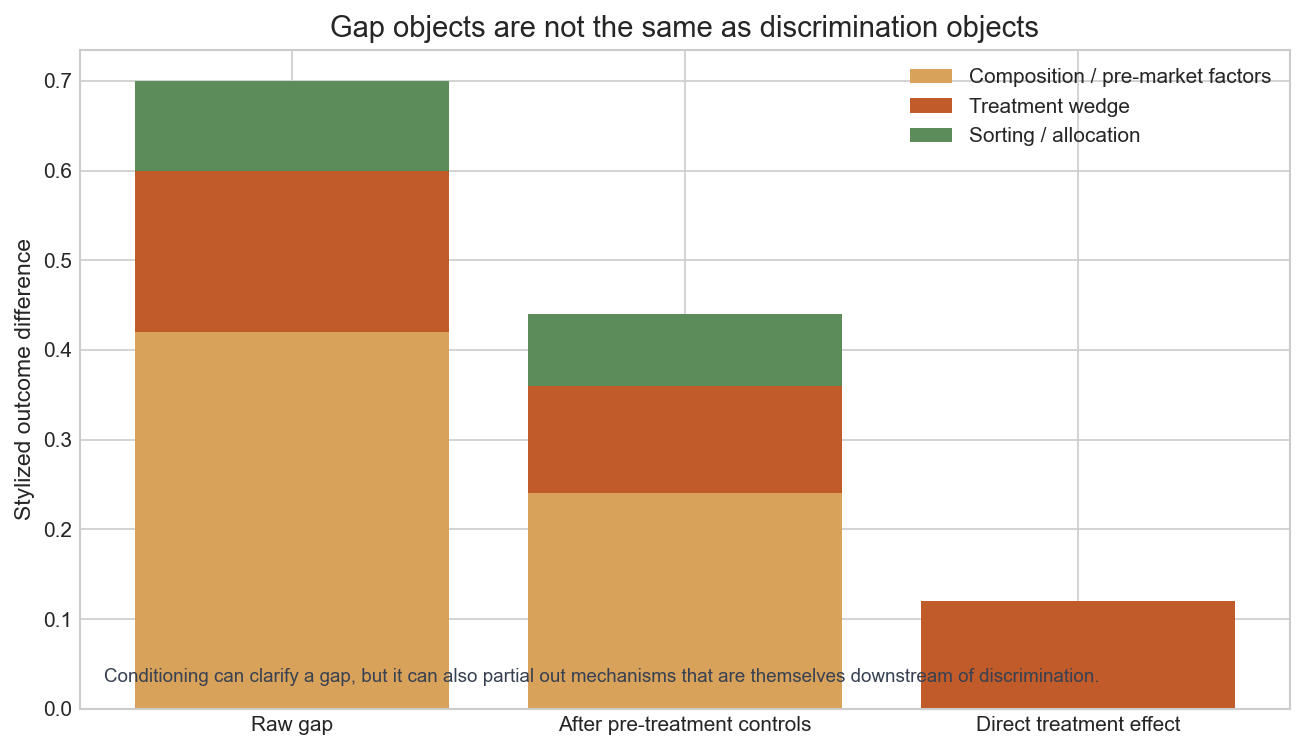
\includegraphics[height=0.74\textheight,keepaspectratio]{09-gap-vs-discrimination-schematic.png}
\end{center}
\end{frame}

\begin{frame}{Mechanism taxonomy}
\begin{itemize}
    \item Taste-based discrimination: group identity enters utility or effective labor cost.
    \item Statistical discrimination: noisy signals lead employers to use group-conditioned beliefs.
    \item Sorting or segmentation: groups are differentially assigned across firms, tasks, occupations, or places.
    \item Similar reduced-form gaps can emerge from very different mechanisms.
\end{itemize}
\end{frame}

\begin{frame}{Mechanism comparison}
\begin{center}
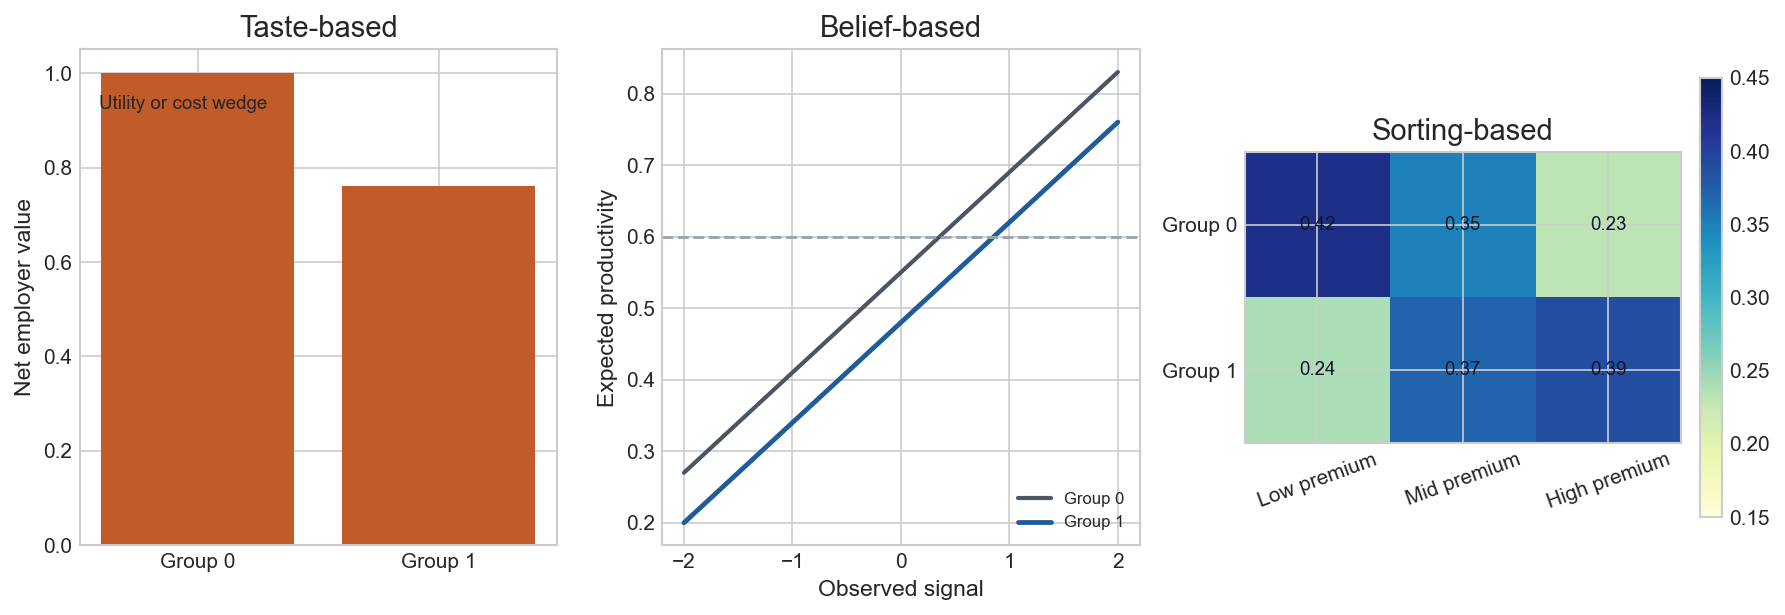
\includegraphics[height=0.72\textheight,keepaspectratio]{09-discrimination-mechanisms.png}
\end{center}
\end{frame}

\begin{frame}{Taste-based discrimination}
\[
\pi_j = p \cdot q_{ij} - w_i - d_j \mathbf{1}\{G_i=1\}
\]

\begin{itemize}
    \item A prejudiced employer behaves as if some workers are more costly.
    \item The wedge can affect hiring, wages, tasks, and retention.
    \item Competition need not eliminate the wedge when search frictions, customer tastes, or concentration matter.
\end{itemize}
\end{frame}

\begin{frame}{Statistical discrimination}
\[
\text{Hire if } \mathbb{E}[a_i \mid s_i, G_i] \geq c_j
\]

\begin{itemize}
    \item Group-conditioned beliefs matter when productivity is imperfectly observed.
    \item The mechanism operates through beliefs, not necessarily prejudice.
    \item Anticipated screening can feed back into schooling, training, and task acquisition.
\end{itemize}
\end{frame}

\begin{frame}{Decomposition logic and bad controls}
\[
\mathbb{E}[Y \mid G=1] - \mathbb{E}[Y \mid G=0]
= \big(\mathbb{E}[X \mid G=1]-\mathbb{E}[X \mid G=0]\big)\beta_0
+ \mathbb{E}[X \mid G=1](\beta_1-\beta_0)
\]

\begin{itemize}
    \item Oaxaca--Blinder style decompositions are descriptive accounting tools.
    \item The unexplained term is not automatically a causal measure of discrimination.
    \item Education, occupation, task, or firm assignment may be bad controls if they are downstream of discrimination.
\end{itemize}
\end{frame}

\begin{frame}{Audit and correspondence identification}
\[
\tau^{cb} = \mathbb{E}[C_i(1) - C_i(0)]
\]

\begin{itemize}
    \item Correspondence designs hold qualifications fixed while changing signaled identity.
    \item The estimand is clean at the callback or contact margin.
    \item It does not by itself recover wage-setting, promotion, or full equilibrium consequences.
\end{itemize}
\end{frame}

\begin{frame}{Audit-study schematic}
\begin{center}
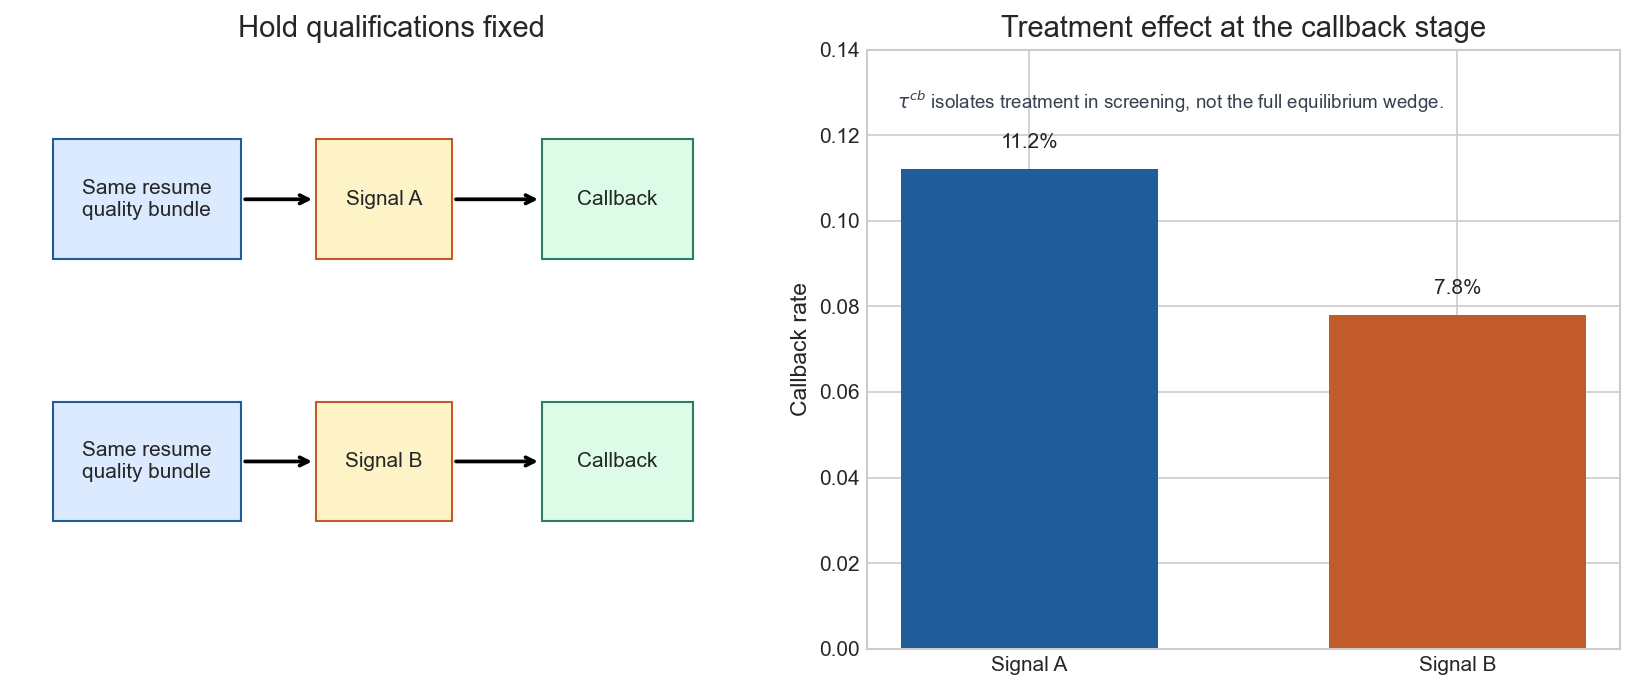
\includegraphics[height=0.72\textheight,keepaspectratio]{09-audit-identification-schematic.png}
\end{center}
\end{frame}

\begin{frame}{Sorting and segmentation}
\[
s_{gf} = \Pr(F_i = f \mid G_i = g)
\]

\begin{itemize}
    \item Differential assignment across firms, occupations, or tasks is itself a discrimination object.
    \item Small within-firm wage gaps can coexist with large between-firm allocation gaps.
    \item This is the direct bridge from Week 8 firm inequality to Week 10 mobility.
\end{itemize}
\end{frame}

\begin{frame}{Sorting heatmap}
\begin{center}
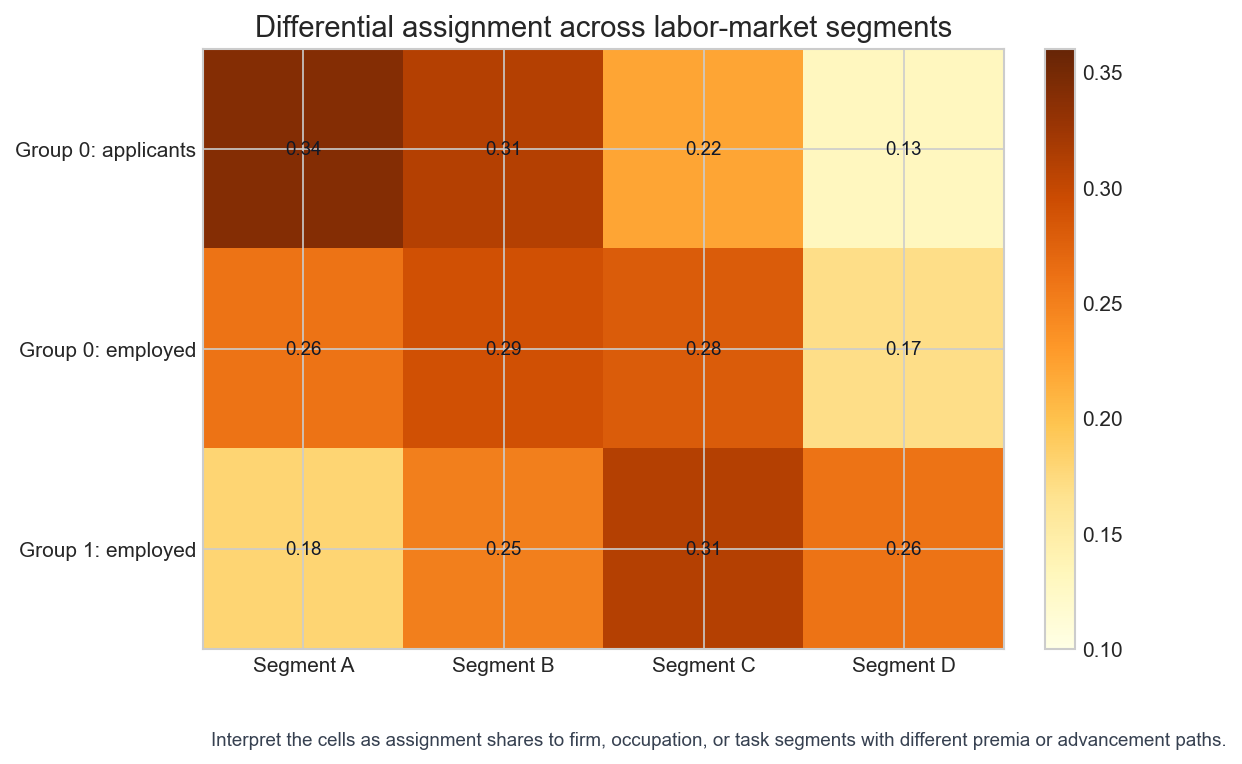
\includegraphics[height=0.72\textheight,keepaspectratio]{09-sorting-segmentation-heatmap.png}
\end{center}
\end{frame}

\begin{frame}{Firm report cards and frontier measurement}
\begin{itemize}
    \item Modern work asks how discrimination varies across employers, not only on average.
    \item Report-card designs combine treatment variation with employer-level heterogeneity.
    \item The frontier challenge is precision: noisy employer rankings can be misleading without shrinkage and uncertainty discipline.
\end{itemize}
\end{frame}

\begin{frame}{Bridge to Week 10}
\begin{itemize}
    \item Week 10 mobility asks how workers move across places, jobs, and generations.
    \item Week 9 shows that the opportunity set they move through may already be segmented.
    \item Mobility can therefore be adjustment, escape, or persistence inside a discriminatory allocation system.
\end{itemize}
\end{frame}

\begin{frame}{Takeaways}
\begin{itemize}
    \item A raw gap is not yet a discrimination estimate.
    \item Taste-based, statistical, and sorting mechanisms can produce similar reduced-form patterns.
    \item Identification depends on the margin: decomposition, audit, and equilibrium designs answer different questions.
    \item Week 9 is the bridge from inequality architecture to segmented mobility and policy design.
\end{itemize}
\end{frame}

\appendix

\begin{frame}{Appendix: optional extension block}
\begin{itemize}
    \item Employer report cards, ranking uncertainty, and firm heterogeneity.
    \item Task-based discrimination and occupational assignment.
    \item Algorithmic screening, monopsony, and discriminatory market power.
\end{itemize}
\end{frame}

\end{document}
